


\begin{applicationActivities}

\begin{definition}
Let \(T: V \rightarrow W\) be a linear transformation.
\(T\) is called \term{injective} or \term{one-to-one} if \(T\) does not map two
distinct vectors to the same place.  More precisely, \(T\) is injective if
\(T(\vec{v}) \neq T(\vec{w})\) whenever \(\vec{v} \neq \vec{w}\).

\begin{center}
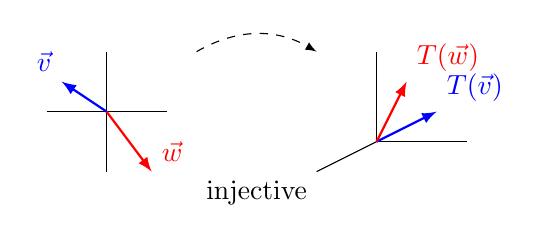
\begin{tikzpicture}[x=0.15in,y=0.15in]
  \begin{scope}[shift={(0,1)}]
    \draw (-2,0) -- (2,0);
    \draw (0,-2) -- (0,2);
    \draw[thick,-latex,blue] (0,0) -- (-1.5,1)
          node[anchor=south east] {\(\vec v\)};
    \draw[thick,-latex,red] (0,0) -- (1.5,-2)
          node[anchor=south west] {\(\vec w\)};
  \end{scope}
  \draw[dashed,-latex] (3,3) to [bend left=30] (7,3);
  \begin{scope}[shift={(9,0)}]
    \draw (0,0) -- (3,0);
    \draw (0,0) -- (0,3);
    \draw (0,0) -- (-2,-1);
    \draw[thick,-latex,blue] (0,0) -- (2,1)
          node[anchor=south west] {\(T(\vec v)\)};
    \draw[thick,-latex,red] (0,0) -- (1,2)
          node[anchor=south west] {\(T(\vec w)\)};
  \end{scope}
  \node[anchor=north] at (5,-1) {injective};
\end{tikzpicture}
\hspace{3em}
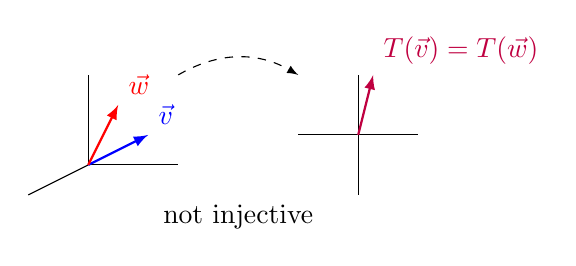
\begin{tikzpicture}[x=0.15in,y=0.15in]
  \begin{scope}[shift={(0,0)}]
    \draw (0,0) -- (3,0);
    \draw (0,0) -- (0,3);
    \draw (0,0) -- (-2,-1);
    \draw[thick,-latex,blue] (0,0) -- (2,1)
          node[anchor=south west] {\(\vec v\)};
    \draw[thick,-latex,red] (0,0) -- (1,2)
          node[anchor=south west] {\(\vec w\)};
  \end{scope}
  \draw[dashed,-latex] (3,3) to [bend left=30] (7,3);
  \begin{scope}[shift={(9,1)}]
    \draw (-2,0) -- (2,0);
    \draw (0,-2) -- (0,2);
    \draw[thick,-latex,purple] (0,0) -- (0.5,2)
          node[anchor=south west] {\(T(\vec v)=T(\vec w)\)};
  \end{scope}
  \node[anchor=north] at (5,-1) {not injective};
\end{tikzpicture}
\end{center}
\end{definition}

\end{applicationActivities}
